\lhead{\emph{Conceptos teóricos}}

\chapter{Conceptos teóricos}

\section{Programación orientada a eventos}
\label{eventdriven}
\section{Computación distribuida}

Un sistema distribuido es aquel conformado por un conjunto de nodos independientes que son percibidos como una entidad única y coherente por el usuario final. Dicha definición implica dos conceptos de importancia en el paradigma:

\begin{itemize}
  \item Autonomía: los diferentes integrantes del sistema cuentan con un alto grado de autonomía entre sí, y por tanto se deben diseñar e implementar mecanismos de comunicación entre los mismos, mecanismos que formarán parte del núcleo del sistema, y cuyo diseño tendrá consecuencias directas en el funcionamiento final del sistema.
  \item Transparencia: Las diferencias entre diferentes nodos suelen ser invisibles para los usuarios finales, así como la gestión de fallos y recuperación y la uniformidad a la hora de interactuar con el sistema. Según \citationneeded las siguientes propiedades del sistema deben contar con un grado de transparencia alto\footnote{En numerosas ocasiones las propiedades de un sistema hacen desfavorable el cumplimiento de todos los requisitos de transparencia. Un ejemplo sería la transparencia de relocación en el sistema DNS.}:
  \subitem \textbf{Acceso}: La forma de almacenamiento y gestión de los recursos e información presentes en el sistema debe ser completamente transparente.
  \subitem \textbf{Localización}: La localización física del sistema no debe ser de relevancia para el uso del mismo.
  \subitem \textbf{Migración}: El cambio de plataforma de un sistema debe ser transparente para el usuario (ejemplo: cambio del sistema operativo).
  \subitem \textbf{Relocación}: El hecho de que un sistema se esté trasladando de un lugar a otro no debe afectar al usuario final.
  \subitem \textbf{Replicación}: El numero de elementos redundantes en un sistema es desconocido para el usuario final.
  \subitem \textbf{Concurrencia}: Un usuario no debe percibir la presencia de otros agentes interactuando con el sistema.
  \subitem \textbf{Gestión de errores}: En caso de fallo, el usuario final no debe percibir el mismo, ni el proceso de recuperación consecuente.
\end{itemize}

Generalmente los sistemas distribuidos son fácilmente escalables gracias a la autonomía de cada nodo, y los mecanismos de transparencia permiten crear sistemas heterogéneos de forma sencilla, en ocasiones apoyados en capas \textit{middleware} que posibilitan dicha transparencia.

Otro concepto importante en el desarrollo de sistemas distribuidos es la ``apertura'' (\textit{openness}) de los mismos. Un sistema ofrece una serie de servicios gracias al uso de un conjunto de reglas conocidas por todos los participantes, generalmente recogidos en estándares de acceso público que definen la sintaxis y semántica de los servicios, conocidos como lenguajes de especificación de interfaz (\textit{Interface Definition Language}). Si dicho lenguaje es definido de forma apropiada, es posible crear diferentes implementaciones del mismo que sean capaces de comunicarse entre sí, incluso ejecutándose sobre máquinas completamente diferentes
%To achieve flexibility in open distributed systems, it is crucial that the system is organized as a collection of relatively small and easily replaceable or adaptable components. This implies that we should provide definitions not only for the highest-level interfaces, that is, those seen "by users and applications, but also definitions for interfaces to internal parts pJ the system and describe how those parts interact. This approach is relatively new. Many older and even contemporary systems are constructed using a monolithic approach in which components  (Tanenbaum, p8)

\subsection{Escalabilidad}

La escalabilidad del sistema en ocasiones se ve afectada por las decisiones de diseño llevadas a cabo. En arquitecturas centralizadas el punto principal del sistema consituye un ``cuello de botella'' evidente que define un límite en el crecimiento del sistema. La disposición geográfica exige una serie de consideraciones adicionales, entre las que se encuentra la latencia del sistema.

\subsection{Algoritmos distribuidos}

Un algoritmo distribuido es aquel que realiza una tarea de forma distribuida, cumpliendo el siguiente conjunto de propiedades:

\begin{itemize}
\item Ningún componente conoce el total de la información sobre el estado del sistema (principio de autonomía).
\item Un componente únicamente puede tomar decisiones basadas en su conocimiento local (principio de autonomía).
\item El fallo de un nodo no provoca el fallo del sistema (transparencia).
\item No hay una asunción implícita de que existe un reloj global.
\end{itemize}

\subsection{Modelos arquitectónicos}

Existe un gran rango de diferentes modelos de construcción de sistemas distribuidos en función de las necesidades a cubrir por el sistema.

%Tanenbaum 2.1

\subsubsection{Clúster}

En general se conoce como clúster al conjunto de nodos homogéneos y dispuestos físicamente en la misma localización, conectados entre sí mediante mecanismos fiables como redes de área local y que cuentan con el mismo conjunto de herramientas (en particular el sistema operativo). Generalmente estos sistemas se componen de nodos de bajo coste, como equipos de escritorio (denominados \textit{Commodity Off-The-Shell})\citationneeded{http://en.wikipedia.org/wiki/Commodity\_computing} y son utilizados para la realización de una única tarea con un coste computacional alto en paralelo.


\write18{wget -O Chapters/Chapter2/Figures/Beowulf.png -nc   http://upload.wikimedia.org/wikipedia/commons/4/40/Beowulf.png?download}

\begin{figure}[H]
\centering
\includegraphics[width=0.7\textwidth]{Chapter2/Figures/Beowulf.png}
\caption{Esquema de un clúster Beowulf, un tipo de clúster}
\label{fig:beowulf}
\end{figure}

\subsubsection{\textit{Grid}}

Una ``rejilla'' (grid) es un sistema distribuido en el que los nodos del sistema no son homogéneos y cuentan con diferentes características. Los mecanismos de transparencia descritos anteriormente son clave para el correcto funcionamiento del sistema y las interconexiones entre los diferentes elementos.


\subsubsection{Sistemas de información distribuida}

\subsubsection{Sistemas descentralizados}

Uno de los problemas de las arquitecturas propuestas es la dependencia de un nodo que actúe de coordinador para el resto de los nodos del sistema.

\subsection{Seguridad}

Las medidas de seguridad a tomar dependen de las propiedades y objetivos propios del sistema: en general sistemas utilizados dentro de una organización y una infraestructura sin interacción con entornos no controlados suelen contar con un número menor de medidas de seguridad que aquellos utilizados en entornos ``hostiles'', y la seguridad depende de la confianza depositada en la administración del sistema. Sin embargo, un sistema de este tipo es vulnerable a ataques internos por parte de usuarios o intrusiones en la infraestructura.

Un sistema integrado en un entorno hostil debe además vigilar cualquier tipo de potencial ataque malicioso y controlar el acceso al sistema de forma más minuciosa.

\subsection{Integridad}

\subsection{Comunicación}

\subsection{Distribución}

Uno de los modelos típicos en el desarrollo de sistemas distribuidos es el ``divide y vencerás'': la división de un problema en múltiples tareas y la distribución de las mismas entre los diferentes componentes del sistema, reagrupando los resultados posteriormente. Dicho paradigma no se aplica únicamente a tarea a realizar, sino también al conjunto de datos sobre el que realizarla, paralelizando una misma operación en diferentes nodos sobre fragmentos del conjunto de datos sobre el que operar, recopilando los datos devueltos y conformando la respuesta final.

\write18{wget -P Chapters/Chapter2/Figures/ -nc http://upload.wikimedia.org/wikipedia/commons/6/6d/Mapreduce.png}

\begin{figure}[H]
\centering
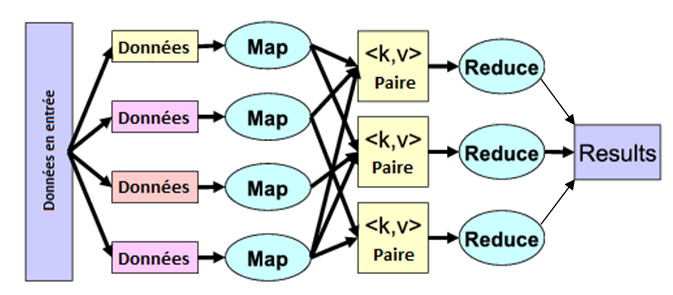
\includegraphics[width=0.7\textwidth]{Chapter2/Figures/Mapreduce.png}
\caption{\textbf{MapReduce} se basa en el principio de la distribución de los datos sobre diferentes nodos (\textit{Map}) y la recopilación de los datos procesados (\textit{Reduce})}
\label{fig:mapreduce}
\end{figure}

\subsection{Autoadministración}

%2.4 SELF -MANAGEMENT IN DISTRIBUTED SYSTEMS 

\section{Paralelización, \textit{threads}}
\section{Multicasting}

\section{WebSockets}

\section{Test-Driven Development}


\section{PAM}

\section{Cross-compiling}

\section{Python}

\lhead{\emph{Dominio del problema}}
\chapter{Dominio del problema}

La utilización de algoritmos distribuidos implica mejoras sustanciales en una gran cantidad de aplicaciones, incrementando la capacidad global de computación de un sistema mediante la unión de varios dispositivos de cómputo que trabajan de como una única unidad indivisible a la vez que mantienen un alto grado de independencia y una tolerancia global a fallos muy alta. Sin embargo, el desarrollo de aplicaciones distribuidas implica el uso de un conjunto de nodos cuyo coste y mantenimiento es costoso.

Dicho aumento de la potencia implica una mayor complejidad en el desarrollo de algoritmos que puedan aprovechar de forma óptima este tipo de sistemas. Varios factores como la sincronización y la comunicación entre partes, o errores tales como condiciones de carrera son mucho más comunes que en otro tipo de aplicaciones. Dichas dircunstancias no solo dificultan el desarrollo de este sistema, sino también la comprensión de los fundamentos básicos de la Computación Distribuida. %cite http://ceit.aut.ac.ir/~amirkhani/Downloads/patterson_book.pdf

Si bien la mayoría de las aplicaciones en las que el paradigma de computación distribuida introduce mejoras suelen exigir una gran capacidad de cálculo, su desarrollo únicamente requiere un conjunto de instancias independientes de un software (sistema operativo, contenedor de servicios...) con las que trabajar. Dicha característica implica que la utilización de nodos de precio reducido (o incluso reutilizados) para el diseño, análisis y evaluación de este tipo de algoritmos constituye una alternativa válida frente a sistemas de precio superior.

Sumada a dicha motivación existe el potencial aprovechamiento de este sistema como herramienta didáctica que facilite el aprendizaje de conceptos como el reparto de procesos, balance de carga o la compartición de recursos en asignaturas centradas en este tipo de conceptos dentro de los planes de estudio de Ingeniería Informática o titulaciones afines.

Con el presente proyecto se plantea la creación de un sistema con estas características aprovechando el bajo coste de los componentes del mismo que permita en primer lugar su utilización como herramienta de análisis y diseño (o incluso su utilización como plataforma definitiva) de aplicaciones distribuidas y en segundo lugar la posibilidad de uso como herramienta educativa.

A la hora de crear el sistema se realiza un análisis de las diferentes alternativas, a fin de escoger la alternativa que mejor satisfaga los objetivos definidos.

Figura: Tabla de alternativas

\section{Objetivos del proyecto}

Este proyecto cuenta con varios objetivos muy diferentes entre sí, que se agrupan en tres categorías:
\begin{itemize}
  \item Arquitectura subyacente\\
  Definición de los componentes hardware a utilizar en el sistema, interconexión de los mismos, soluciones de alimentación eléctrica, almacenamiento\dots.
  \item Servicios a proveer\\
  Conjunto de servicios que podrán ser aprovechados por diferentes clientes para explotar la capacidad de cálculo de las máquinas.
  \item Componente didáctico\\
  Creación de aplicaciones, herramientas y documentación como alternativa a las instalaciones típicas utilizadas actualmente.
\end{itemize}

\section{Definiciones}

\subsection{Definición del dominio del problema}

El sistema se ubica en una Facultad universitaria con aproximadamente 600 alumnos\citationneeded con varias asignaturas en las que se imparten áreas de conocimiento relacionados con la Computación Distribuida, en particular las asignaturas \textbf{Arquitectura de Computadores} y \textbf{Sistemas Distribuidos} \cite{DIA15GuiaAcademica}.

\subsection{Modelado del sistema actual}

La Facultad cuenta con varias aulas y laboratorios informáticos donde los alumnos disponen de la intraestructura necesaria para realizar los ejercicios y prácticas asignadas. Dichos espacios permiten utilizar cualquier equipo como nodo, pues se integran en la misma red, siendo incluso factible la comunicación directa entre equipos situados en diferentes aulas o incluso edificios. La conexión es relativamente rápida, contando con un cableado capaz de soportar teóricamente transferencias de hasta 100Mb/s de forma bidireccional (\textit{full-duplex}) (\textbf{Cita requerida}). La gestión de un sistema de autenticación se realiza mediante el protocolo LDAP (\textit{Lightweight Directory Access Protocol}) \cite{RFC4516-comment}, contando con un sistema de ficheros centralizado que permite acceder a la información de un usuario desde cualquier equipo, facilitando las tareas de replicación de la información entre nodos.

La mayoría de las prácticas asignadas a los alumnos son desarrolladas en el lenguaje \textbf{Java}, ya conocido por la totalidad de los estudiantes gracias a asignaturas previamente cursadas (\textbf{Cita requerida}) y que facilita el despliegue y la compatibilidad entre diferentes equipos de trabajo sustancialmente. En ocasiones es necesario el uso de lenguajes como C y se plantean alternativas a \textit{Java} como Python o C\#.

\paragraph{Problemas conocidos}

Si bien la infraestructura existente es capaz de proveer a los estudiantes de los recursos necesarios, identificamos una serie de problemas inicialmente:

\begin{itemize}
  \item Cada grupo de alumnos necesita tres estaciones de trabajo para poder realizar algunos de los ejercicios propuestos.
  \item El servidor LDAP constituye un ``cuello de botella'', pues todos los alumnos acceden a él de forma intensiva, provocando el fallo por exceso de peticiones del mismo.
  \item Las técnicas de programación utilizadas hasta la fecha tienen un rendimiento bajo y son en ocasiones relativamente complejas.
\end{itemize}

\subsection{Identificación de usuarios participantes}

\begin{itemize}

  \item Estudiantes de tercero y cuarto curso del Grado en Ingeniería Informática.
  \item Doctentes de las asignaturas Arquitectura de Computadores y Sistemas Distribuidos.
  \item Administradores del Sistema.
\end{itemize}

\section{Identificación de las necesidades de cada parte}
\subsection{Necesidades de los alumnos}

\begin{itemize}
  \item Entorno de trabajo sencillo que agilice el desarrollo de sus prácticas.
  \item Posibilidad de observar los resultados de las ejecuciones de forma sencilla.
  \item Facilidades para el despliegue de los diferentes ejecutables en todas las máquinas, así como el consumo de los servicios que estos implementen.
\end{itemize}

\subsection{Necesidades de los docentes}

\begin{itemize}
  \item Entorno versátil sobre el cual puedan llevarse a cabo la totalidad de las prácticas y ejercicios propuestos, aportando si es posible algún tipo de ventaja sobre el sistema en uso.
\end{itemize}

\subsection{Administrador}

\begin{itemize}
  \item Sistema integrable en la intraestructura actual cuyo mantenimiento sea sencillo y cuyo enfoque garantice la escalabilidad y su durabilidad.
\end{itemize}

\section{Propuestas para la búsqueda de necesidades}

\begin{itemize}
  \item Encuestas o entrevistas a todas las partes.
  \item Evaluación de la experiencia de uso en las diferentes etapas de desarrollo del sistema.
\end{itemize}

\section{Identificación de requisitos}

\subsection{Requisitos de almacenamiento de la información}

\begin{itemize}
  \item Gestión de usuarios (credenciales de autenticación)
  \item Gestión de los datos de cada usuario
  \item \textit{Logs} del sistema
\end{itemize}

\subsection{Identificación de requisitos funcionales}


\subsection{Identificación de requisitos no funcionales}

\begin{itemize}
  \item El \textit{software} debe ser mantenible y robusto\footnote{Siendo dicha robustez garantizada mediante el uso de \textit{software} utilizado por una base de usuarios significativa, una arquitectura conocida, pruebas realizadas sobre él o un equipo de desarrollo en activo, entre otras}.
  \item Reducción de los costes de desarrollo.
  \item Definición de los protocolos de comunicación.
  \item Definición de los protocolos de seguridad y confidencialidad.
  \item Definición de la interacción con el usuario.
  \item Integridad del sistema y fiabilidad (\textit{uptime}, recuperación frente a fallos).
  \item Productos a crear.
  \item Compatibilidad con las prácticas y ejercicios.
\end{itemize}

\section{Evaluación de alternativas}
\label{alternativas}
A la hora de evaluar las diferentes opciones que satisfagan los requisitos descritos, se consideran los siguientes aspectos:

\begin{itemize}
  \item Coste económico.
  \item Prestaciones técnicas (potencia de procesamiento, entrada/salida, capacidad de almacenamiento,facilidad de interconexión con otros materiales...).
  \item Facilidad de trabajo y de aprendizaje (documentación disponible, proyectos similares ya realizados, conocimiento sobre la plataforma en cuestión...).
  \item Escalabilidad del sistema.
  \item Necesidades de mantenimiento del sistema.
  \item Consumo del sistema (consumo eléctrico).
  \item Obsolescencia del sistema (número de años en los que el sistema podrá ser actualizado (tanto en hardware como software) y será capaz de seguir siendo una herramienta adecuada para el propósito planteado).

\end{itemize}

\subsection{Propuesta de solución: Virtualización de entornos de trabajo}

Crear un conjunto de nodos virtuales dentro de una máquina que simulen un sistema distribuido

\paragraph{Ventajas intrínsecas de la solución}

Simplificación del sistema (reduce las necesidades de adquisición y mantenimiento de hardware).
Gestión de varias partes del sistema (sistema de ficheros centralizado, gestión de usuarios...) de forma mas sencilla. El coste se reduce significativamente.

\paragraph{Inconvenientes intrínsecos del sistema}

No se exploran apenas las posibilidades de un sistema distribuido formado por varios equipos físicamente independientes.

\paragraph{Facilidad de trabajo y curva de aprendizaje}

Si bien el trabajo con cada una de las instancias es previsiblemente sencillo, debido a la eliminación de la gran parte del mantenimiento de la capa física subyacente, el uso de este tipo de sistema requiere una etapa de formación previa en materia de virtualización.

\paragraph{Prestaciones técnicas}

Las prestaciones técnicas con las que se contaría, de llevarse a cabo este proyecto, son las de los equipos ya dispuestos para fines similares a este en el Centro: %TODO: Andrés. 

\paragraph{Coste econonómico}

El coste econónomico es muy reducido si ya se cuenta con los equipos a utilizar y las licencias \textit{software} que fueran necesarias para realizar la virtualización.

\paragraph{Escalabilidad del sistema}

Dependiente de las capacidades de virtualización del equipo disponible, y el número de nodos y usuarios a gestionar (previsiblemente alto)

\paragraph{Necesidades de mantenimiento}

Las necesidades propias de un sistema GNU/Linux junto a las específicas de la virtualización de los equipos.

\paragraph{Consumo energético del sistema}
\paragraph{Obsolescencia del sistema}

\paragraph{Material con el que se cuenta actualmente}
Se plantea el aprovechamiento de equipos pertenecientes a la Universidad, por lo que se estima un coste muy pequeño a la hora de adquirir material.
\paragraph{Otras características}

\paragraph{Análisis coste/beneficio}

Si bien el coste de esta solución es muy atractivo, presenta una serie de carencias que dificultan significativamente el desarrollo del sistema en el mismo. 


\subsection{Propuesta de solución: Clúster con equipos de escritorio}

Se plantea la reutilización de equipos de escritorio pertenecientes a la Universidad que ya no se encuentran en uso (debido a su renovación, falta de potencia como PC...) para la creación de este sistema.

\paragraph{Ventajas intrínsecas de la solución}
La potencia del sistema es mucho mayor que la de cualquier otra solución considerada viable. Se reduce dramáticamente el coste de adquisición de material y permite dar un nuevo ciclo de vida a material universitario.
La arquitectura es conocida y fiable.

\paragraph{Inconvenientes intrínsecos del sistema}

No se exploran las características únicas de otros sistemas menos ``convencionales'', tales como la utilización de sistemas embebidos. El consumo energético es mayor, existe una mayor demanda de espacio, que puede dificultar la implementación de diferentes aplicaciones didácticas ya planteadas como objetivo funcional del sistema.

\paragraph{Facilidad de trabajo y curva de aprendizaje}

Soporte completo de casi la totalidad de las distribuciones de GNU/Linux.
Las necesidades de manipulación de hardware se minimizan.

\paragraph{Prestaciones técnicas}
Arquitectura x86/x64
Entre 2 y 4 GB de memoria
Conectividad Ethernet, USB
Almacenamiento en disco duro
\paragraph{Coste econonómico}

El coste económico de dichos equipos es prácticamente nulo, pues ya se cuenta con los mismos y su utilización no exige la adquisición de sustitutos, pues ya habían sido retirados de su uso.

\paragraph{Escalabilidad del sistema}

Dependiente únicamente del coste económico de la adquisición de nuevos equipos, o de la disponibilidad de equipos desechados.

\paragraph{Necesidades de mantenimiento}

Las necesarias en cualquier sistema GNU/Linux y las específicas del montaje dado (en materia de refrigeración, gestión de cableado, etcétera).

\paragraph{Consumo energético del sistema}

El típico de cualquier equipo de escritorio.

\paragraph{Obsolescencia del sistema}

Estos equipos tienen una antigüedad de aproximadamente 4 años. Dicha edad no impide que sean capaces de utilizar aplicaciones actuales, y en general no se prevé la incompatibilidad con ninguna aplicación.

\paragraph{Material con el que se cuenta actualmente}
La Facultad de Ciencias ya dispone de los equipos, pues se plantea la reutilización de los mismos

\paragraph{Otras características}

\paragraph{Análisis coste/beneficio}

Si bien el coste de estos equipos es prácticamente nulo, dicho atractivo contrasta con los potenciales problemas que el uso de estos sistemas puede implicar (dificultad de desarrollo de objetivos funcionales, uso de sistemas convencionales en detrimento de soluciones más innovadoras\dots).

\subsection{Clúster con equipos embebidos multimedia }

Utilización de equipos embebidos diseñados para aplicaciones multimedia en el sistema (ejemplos son Chromecast, Apple TV, Amazon Fire TV...)

\paragraph{Ventajas intrínsecas de la solución}

Relacion potencia/precio presumiblemente superior a soluciones de coste similar como las placas Raspberry Pi.

\paragraph{Inconvenientes intrínsecos del sistema}

Dificultad de conexión (generalmente la conexión a red se realiza de forma inalámbrica, ausencia casi absoluta de cualquier conexión cuya finalidad no sea la emisión de vídeo o conexión con sistemas de almacenamiento mediante USB), falta de puertos GPIO, I2C...

\paragraph{Facilidad de trabajo y curva de aprendizaje}
Es difícil determinar la viabilidad de esta solución, pues no se cuenta con experiencia previa ni una documentación amplia al respecto.
Es probable que sea necesaria la manipulación del sistema a muy bajo nivel. Lo cual incrementa el grado de complejidad de la solución.

\paragraph{Prestaciones técnicas}
Arquitectura ARM
2 núcleos a 1.2 GHz
512 MB de RAM
Almacenamiento: 2 GB no expandibles
Alimentación por microUSB

\paragraph{Coste econonómico}

El coste de estos equipos es reducido, generalmente inferior a 30 € por unidad.

\paragraph{Escalabilidad del sistema}

Dependiente del coste de adquisición de nuevos equipos y las facilidades de interconexión de la plataforma (previsiblemente compleja, debido a la ausencia de sistemas de interconexión más allá de WiFi)

\paragraph{Necesidades de mantenimiento}

Dependiente del número de modificaciones que se realicen a las capas más bajas. En el peor de los casos puede que el administrador del sistema tenga que someterse a una etapa de formación para realizar un mantenimiento adecuado del sistema sin depender de desarrolladores previos.
Las derivadas del mantenimiento de un sistema Linux sumadas a posibles problemas de interconexión si se utiliza una red inalámbrica (conexión a  la LAN de la infraestructura local, interferencias...).

\paragraph{Consumo energético del sistema}

El diseño de estos equipos está orientado a la reducción del consumo, por lo que se estima reducido.

\paragraph{Obsolescencia del sistema}

Difícil de determinar: no se cuenta con una gran cantidad de software para este tipo de sistemas más allá de las aplicaciones multimedia. No obstante, el sistema subyacente es conocido (Linux)

\paragraph{Material con el que se cuenta actualmente}

No se dispone de material de estas o similares características

\paragraph{Otras características}

\subsection{Clúster con equipos embebidos multimedia }

Utilización de equipos embebidos diseñados para aplicaciones multimedia en el sistema (ejemplos son Chromecast, Apple TV, Amazon Fire TV...)

\paragraph{Ventajas intrínsecas de la solución}

Relacion potencia/precio presumiblemente superior a soluciones de coste similar como las placas Raspberry Pi.

\paragraph{Inconvenientes intrínsecos del sistema}

Dificultad de conexión (generalmente la conexión a red se realiza de forma inalámbrica, ausencia casi absoluta de cualquier conexión cuya finalidad no sea la emisión de vídeo o conexión con sistemas de almacenamiento mediante USB), falta de puertos GPIO, I2C...

\paragraph{Facilidad de trabajo y curva de aprendizaje}
Es difícil determinar la viabilidad de esta solución, pues no se cuenta con experiencia previa ni una documentación amplia al respecto.
Es probable que sea necesaria la manipulación del sistema a muy bajo nivel. Lo cual incrementa el grado de complejidad de la solución.

\paragraph{Prestaciones técnicas}
Arquitectura ARM
2 núcleos a 1.2 GHz
512 MB de RAM
Almacenamiento: 2 GB no expandibles
Alimentación por microUSB

\paragraph{Coste econonómico}



\paragraph{Escalabilidad del sistema}
Dependiente del coste de adquisición de nuevos equipos y las facilidades de interconexión de la plataforma (previsiblemente compleja, debido a la ausencia de sistemas de interconexión más allá de WiFi)

\paragraph{Necesidades de mantenimiento}

Dependiente del número de modificaciones que se realicen a las capas más bajas. En el peor de los casos puede que el administrador del sistema tenga que someterse a una etapa de formación para realizar un mantenimiento adecuado del sistema sin depender de desarrolladores previos.
Las derivadas del mantenimiento de un sistema Linux sumadas a posibles problemas de interconexión si se utiliza una red inalámbrica (conexión a  la LAN de la infraestructura local, interferencias...).

\paragraph{Consumo energético del sistema}



\paragraph{Obsolescencia del sistema}

Difícil de determinar: no se cuenta con una gran cantidad de software para este tipo de sistemas más allá de las aplicaciones multimedia. No obstante, el sistema subyacente es conocido (Linux)

\paragraph{Material con el que se cuenta actualmente}

No se dispone de material de estas o similares características

\paragraph{Otras características}

\subsection{Clúster con Raspberry Pi}

Utilizar la plataforma de hardware libre Raspberry Pi para la creación del sistema, disponiendo los diferentes equipos en un pequeño ``rack'' con un sistema de alimentación propio centralizado y una conexión directa a la infraestructura local.

\paragraph{Ventajas intrínsecas de la solución}
Existen varias soluciones similares bien documentadas.
El hardware es flexible, barato y el consumo es pequeño.
Gran comunidad de desarrolladores alrededor de la plataforma.

\paragraph{Inconvenientes intrínsecos del sistema}

La potencia del sistema es pequeña (ver seccion prestaciones técnicas)

\paragraph{Facilidad de trabajo y curva de aprendizaje}

Ya se cuenta con experiencia en el manejo de estas placas.
Amplia documentación de las prestaciones de la misma.
Proyectos similares ya realizados.
Soporte completo de varias distribuciones de GNU/Linux

\paragraph{Prestaciones técnicas}

Arquitectura ARM
Entre 512 MB y 1 GB de memoria
1 o 4 Núcleos a 700 o 900 MHz (overclock a 1 GHz de forma segura)
Conectividad Ethernet, I2C, GPIO
Alimentación por microUSB/GPIO
Almacenamiento entre 1 GB y 256 GB mediante tarjetas MicroSD/SD

\paragraph{Coste econonómico}

\paragraph{Escalabilidad del sistema}

Dependiente únicamente del coste económico de la adquisición de nuevos equipos

\paragraph{Necesidades de mantenimiento}

Las mismas que cualquier sistema GNU/Linux de iguales características.
Pueden surgir problemas con la fuente de alimentación, dado que es una solución propia.

\paragraph{Consumo energético del sistema}

Variable según modelo, entre 3 y 4 W, con 5V de tensión y un amperaje variable entre 0.6 y 0.8 A

\paragraph{Obsolescencia del sistema}

El software de terceros (sistema operativo, bibliotecas, etc) a incluir está respaldado por una comunidad extensa que provee actualizaciones de forma continua, por lo que previsiblemente el sistema podrá estar actualizado durante varios años.
Las necesidades que el sistema cubre no demandarán previsiblemente una mayor potencia de cálculo.
 

\paragraph{Material con el que se cuenta actualmente}

El Departamento de Informática y Automática cuenta con varios de estos equipos se plantea la reutilización de los mismos

\paragraph{Otras características}



\subsection{Elección de la solución}

\subsection{Raspberry Pi: Elección de las características básicas del sistema}
Comparativa de las características relevantes de los diferentes modelos de Raspberry Pi.
Quedan descartados los modelos A y A+ por la carencia de puerto Ethernet (amén de otras características necesarias).
\begin{landscape}
\begin{table}[h]
\begin{tabular}{|p{3cm}|p{6cm}|p{6cm}|p{6cm}|}
\hline
 & Modelo B & Modelo B+ & Modelo B 2\\ \hline
Procesador & ARMv6 1 Núcleo, 700 MHz (safe overclock hasta 1GHz) & ARMv6 1 Núcleo, 700 MHz (safe overclock hasta 1GHz) & ARMv7 4 Núcleos a 900 MHz \\ \hline
Memoria           & 512 MB compartidos con GPU & 512 MB compartidos con GPU & 1 GB compartido con GPU\\ \hline
Evaluación de rendimiento con LINPACK \cite{hackaday:benchmarkpi2,gist:linpackbenchmark,elinux:benchmark} & 40.64 & 40.64 & 92.88\\ \hline
Conexiones & 2 USB, GPIO de 8 pines. Ethernet 10/100 & 4 USB, GPIO de 17 pines. Ethernet 10/100 & 4 USB, GPIO de 17 pines. Ethernet 10/100\\ \hline
Consumo medio \citationneeded & 700 mA, 5 V (3.5 W) & 600 mA, 5 V (3 W) & 800 mA, 5 V (4 W)\\ \hline
Almacenamiento & SD & MicroSD & MicroSD\\ \hline
Alimentación & Mediante MicroUSB o los pines GPIO & Mediante MicroUSB o los pines GPIO &Mediante MicroUSB o los pines GPIO\\ \hline
Sistemas operativos compatibles & 
%\begin{itemize}
% \setlength\itemsep{0.005em}
Archlinux ARM, OpenELEC, Puppy Linux, Raspbmc, RISC OS, Raspbian, XBian, openSUSE, Slackware ARM, FreeBSD, Plan 9, Kali Linux, Sailfish OS, Pidora (Fedora Remix), Lista completa en \citationneeded & Los mismos que para el modelo B & Hasta la fecha, únicamente:
%\end{itemize} 

%\begin{itemize}

Ubuntu Snappy Core, Raspbian, OpenELEC, RISC OS, Según la web de ArchLinux, también soporta este sistema operativo \footnote{\href{http://archlinuxarm.org/platforms/armv7/broadcom/raspberry-pi-2}{archlinuxarm.org/platforms/armv7/broadcom/raspberry-pi-2}} \\
%\end{itemize}\\ 
\hline % 

Otros & Modelo descatalogado, el soporte oficial y proporcionado por la comunidad probablemente será menor que para los modelos más recientes en el futuro. &  & Lleva poco tiempo en el mercado (apenas un mes). Se conocen pequeños fallos en el hardware (fotosensibilidad de algún componente).\\ \hline

\end{tabular}
\end{table}
\end{landscape}


% \verb{[1] Software para Raspberry Pi http://en.wikipedia.org/wiki/Raspberry_Pi#Software
% [3] Comparativa de placas https://learn.adafruit.com/embedded-linux-board-comparison/performance
% [4] Comparativa de modelos (B+ contra Rev 2) https://learn.adafruit.com/introducing-the-raspberry-pi-2-model-b/performance-improvements

% [8]  RasPiTV - 
% How Much Less Power does the Raspberry Pi B+ use than the old model B? http://raspi.tv/2014/how-much-less-power-does-the-raspberry-pi-b-use-than-the-old-model-b}
\begin{landscape}
\subsection{Elección del sistema operativo}
\label{os:evaluation}
\begin{table}[h]
\begin{tabular}{|p{2cm}|p{4cm}|p{5cm}|p{3cm}|p{4cm}|p{4cm}|}
\hline
Nombre & Enfoque & Características notables & Ventajas & Inconvenientes & Software disponible\\ \hline
ArchLinux ARM & Distribucion ligera centrada en el minimalismo y la disponibilidad de software novedoso. Requiere sin embargo que el usuario conozca el entorno GNU/Linux antes de utilizarlo & Muy optimizado con un ciclo de desarrollo que permite contar con software puntero en poco tiempo & Eficiente, gran comunidad alrededor, relativamente sencillo de utilizar & En ocasiones puede ser complejo su uso. Ya no se incluye en las distribuciones por defecto de la Fundacion Raspberry Pi, lo cual puede suponer falta de soporte oficial & 8700 paquetes disponibles en los repositorios oficiales, más pequeño que para otras distribuciones, si bien no se ha encontrado aun software no compatible\\ \hline

Ubuntu Snappy Core & Centrado en la facilidad de uso & Es la distribución más popular (en equipos de escritorio) con gran cantidad de paquetes disponible & Fácil de configurar, gran cantidad de soporte & Aún no ha sido probado en la Raspberry de forma intensiva.El rendimiento de ubuntu suele ser menor al de otros sistemas operativos debido a la gran cantidad de paquetes incluidos por defecto. & \\ \hline 

Raspbian & & & & &\\ \hline
\end{tabular}
\end{table}
\end{landscape}

\begin{landscape}
\begin{table}[h]
\begin{tabular}{|p{2cm}|p{4cm}|p{5cm}|p{3cm}|p{4cm}|p{4cm}|}
\hline
Nombre & Enfoque & Características notables & Ventajas & Inconvenientes & Software disponible\\ \hline

RISC OS & Diseñado específicamente para la arquitectura ARM, aprovechando las posibilidades de dicha arquitectura & Eficiente, basado en el RISCOS original, incluyendo características del mismo. Sistema monousuario con multitarea cooperativa (en contraste con multihilo o multitarea apropriativa) & Muy eficiente & No esta basado en un sistema conocido previamente. Relativamente desfasado en cuanto a la arquitectura del Sistema Operativo. El software suele ser programado en BBC BASIC & \\ \hline

Gentoo & Diseñado para permitir la personalización del sistema al máximo nivel posible & Enfocado en la personalizacion, siendo el sistema compilado en la maquina sobre la que se va a utilizar en vez de ser descargado como archivo binario & Permite ser modificado de forma sencilla & Poco soportado en Raspberry Pi & \\ \hline

Windows 10 & Diseñado para el paradigma IoT & Sencillo de utilizar, con soporte (previsiblemente) del \textit{framework} .NET & Aún no se encuentra disponible\cite{windows10raspberry}. Esta diseñado para un proposito especifico. No compatible con software para Linux de forma nativa & & \\ \hline

\end{tabular}
\end{table}
\end{landscape}


\section{Propuesta de solución definitiva}

En función de la evaluación llevada a cabo se extraen las siguientes decisiones de diseño que conforman la propuesta de solución definitiva:

\subsection{Hardware}

Todo el sistema se construirá sobre placas \textbf{Raspberry Pi} debido a su alta versatilidad, gran potencia de cálculo, interfaces de comunicación, soporte por parte de las diferentes comunidades de desarrolladores y consumo eléctrico.

\subsection{Sistema operativo}

El sistema operativo a utilizar será \textbf{Arch Linux ARM}, debido a la gran comunidad de soporte con la que cuenta, compatibilidad con la gran mayoría de componentes presentes en un sistema GNU/Linux y modelo arquitectónico que apuesta por la simplicidad del sistema, \textit{limpieza} arquitectónica y eficiencia.

\subsection{Herramientas de desarrollo a utilizar}

Se plantea el uso del lenguaje de programación Python como herramienta principal de desarrollo, debido a su potencia de cálculo y simplicidad, que permite crear aplicaciones que consuman pocos recursos (aspecto vital, máxime cuando se utilizará sobre un sistema con un \textit{hardware} poco potente) de forma sencilla y rápida.